\section{Experiment Design}
\label{sec:experiment}

This section describes the experiment design. The study was approved by the university's Institutional Review Board (IRB). 

\subsection{Participant Recruitment}
This study recruited 202 Amazon Mechanical Turk (MTurk) participants using stratified sampling. The system screened participants based on their age, gender, household income, and education level to assure a balanced demographic within each experiment condition while randomly assigning participants to these conditions. This approach aimed to mitigate imbalanced participation demographics~\cite{redmilesHowWellMy2019}.

\begin{figure}[t]
    \centering
    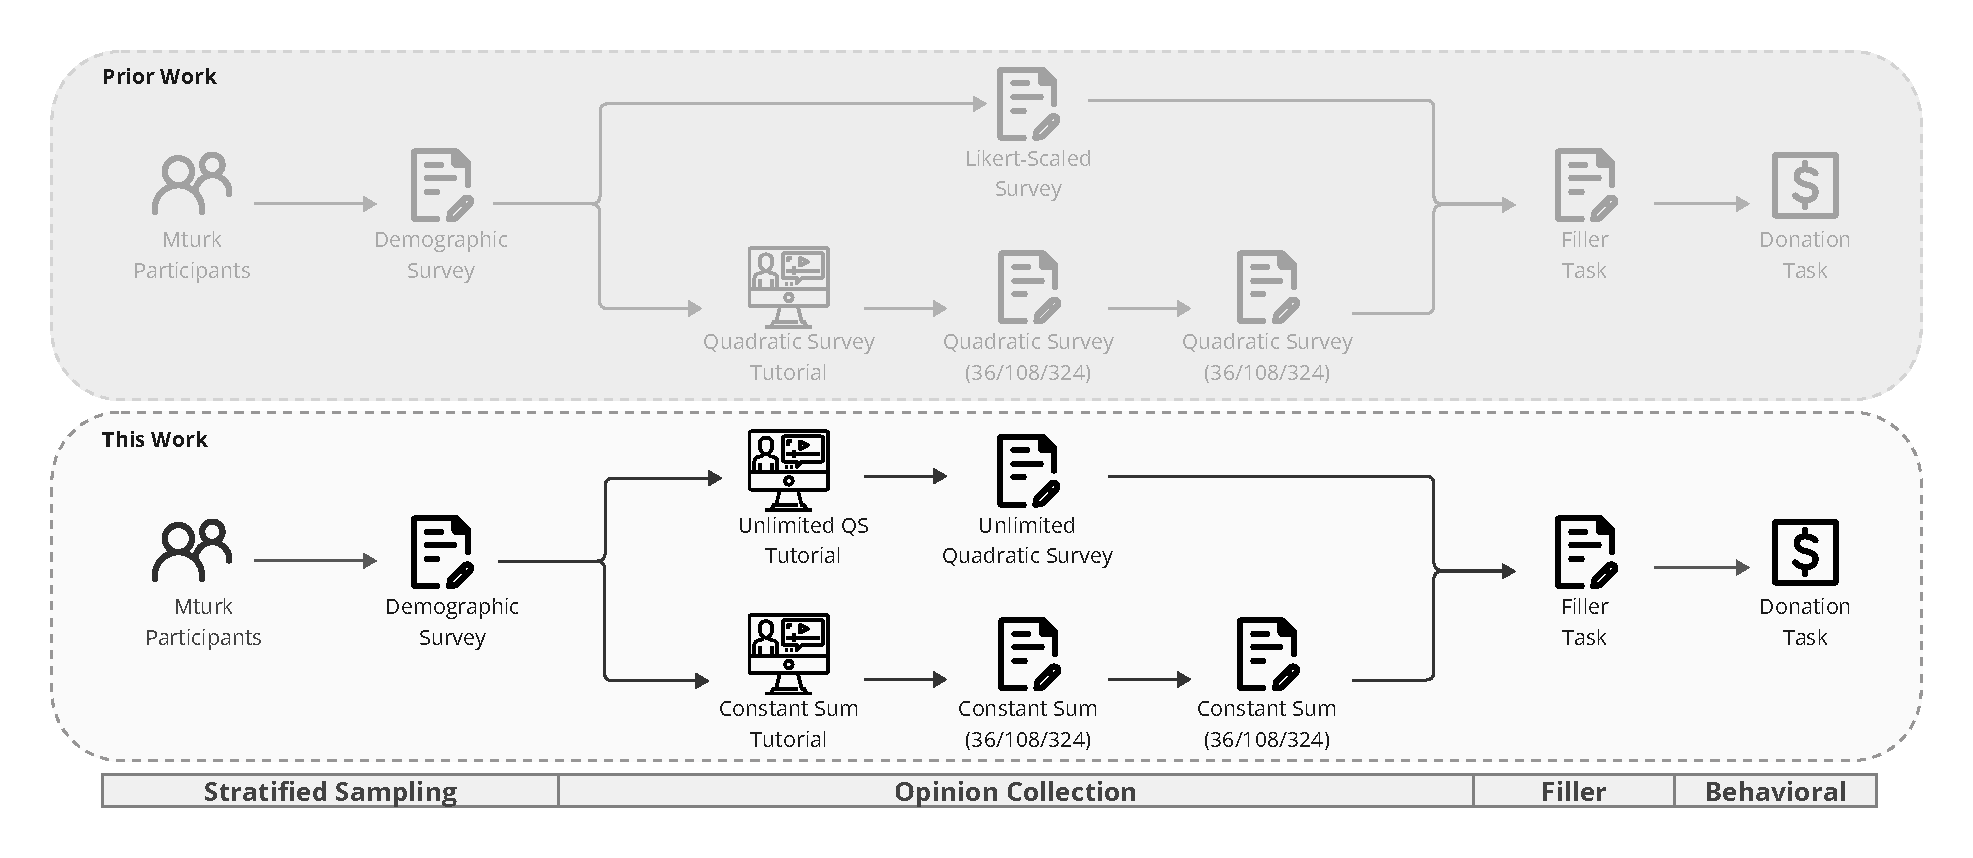
\includegraphics[width=\textwidth]{content/image/whyqs_exp_flow.pdf}
    \caption{Experiment overview. Our study covers the dotted box beneath, mirroring prior research only differing the type of surveys involved during the opinion collection section. The bar below highlights the four parts of the study: sampling, opinion collection, filler task, and the behavioral task.}
    \label{fig:experiment}
\end{figure}

\subsection{Experiment Design}
To ensure comparable data with prior study~\cite{chengCanShowWhat2021}, this study followed the same between-subject experimental design and altered the open sourced software to create two more conditions, creating four new experimental data. We highlight key procedures and alternations we made to the original methodology and redirect choice of surveying method, and the choice of donation as a task, to prior studies for justification. Figure~\ref{fig:experiment} shows how our study fits into the prior work and the overall experiment flow.

\paragraph{Additional Experimental Conditions}
We added four additional experimental conditions presented as two groups, UQS or the LS. The LS group was further divided into three conditions with different budgets:

\begin{itemize}
    \item Unlimited QS (UQS): Participants experience quadratic costs without budget constraints, isolating the effect of cost scaling.
    \item Linear Survey with 18 Credits (LS18): A small-budget linear-cost condition testing the effect of budget constraints.
    \item Linear Survey with 54 Credits (LS54): A medium-budget version allowing greater expressiveness.
    \item Linear Survey with 162 Credits (LS162): A high-budget condition assessing whether increased budgets improve alignment.
\end{itemize}

UQS's isolates the effect of budget constraints while LS isolates the effect of the quadratic cost function cost function. Participants assigned to the LS condition completed two randomly selected LS conditions.

To match the expressiveness of 5-point Likert scales, we allocated 2 credits per option, allowing participants to express moderate intensity in either direction. With 9 options, this yields 18 credits for the LS18 condition. We then scaled budgets using $O(K)$, $O(K^{1.5})$, and $O(K^2)$ to create LS18, LS54, and LS162, respectively—for example, $2 \times 9^{1.5}=54$ in LS54. This isolates the effect of budget constraints under a linear cost structure.

\subsubsection{Survey content}
The study frames the survey as a public resource allotment task, where participants express preferences across 9 societal issues such as education, environment, or health. Participants would express their degree of preferences in number of votes, positive or negatively under the mechanism of UQS or LS.

\subsubsection{Surveying process and interface}
Participants in both groups were first introduced to the survey and how to use it via a video tutorial that we recorded. To assure their understanding of these mechanism, participants were asked to complete a quiz with 5 multiple-choice questions. Participants were required to answer at least 3 questions correctly to continue with the study. We altered the questions based on the survey mechanisms. The interface for both UQS and LS are shown in~\Cref{fig:extended_interface}.

% create a side by side figure using subfigure

\begin{figure}
    \centering
    \begin{subfigure}{0.47\textwidth}
        \centering
        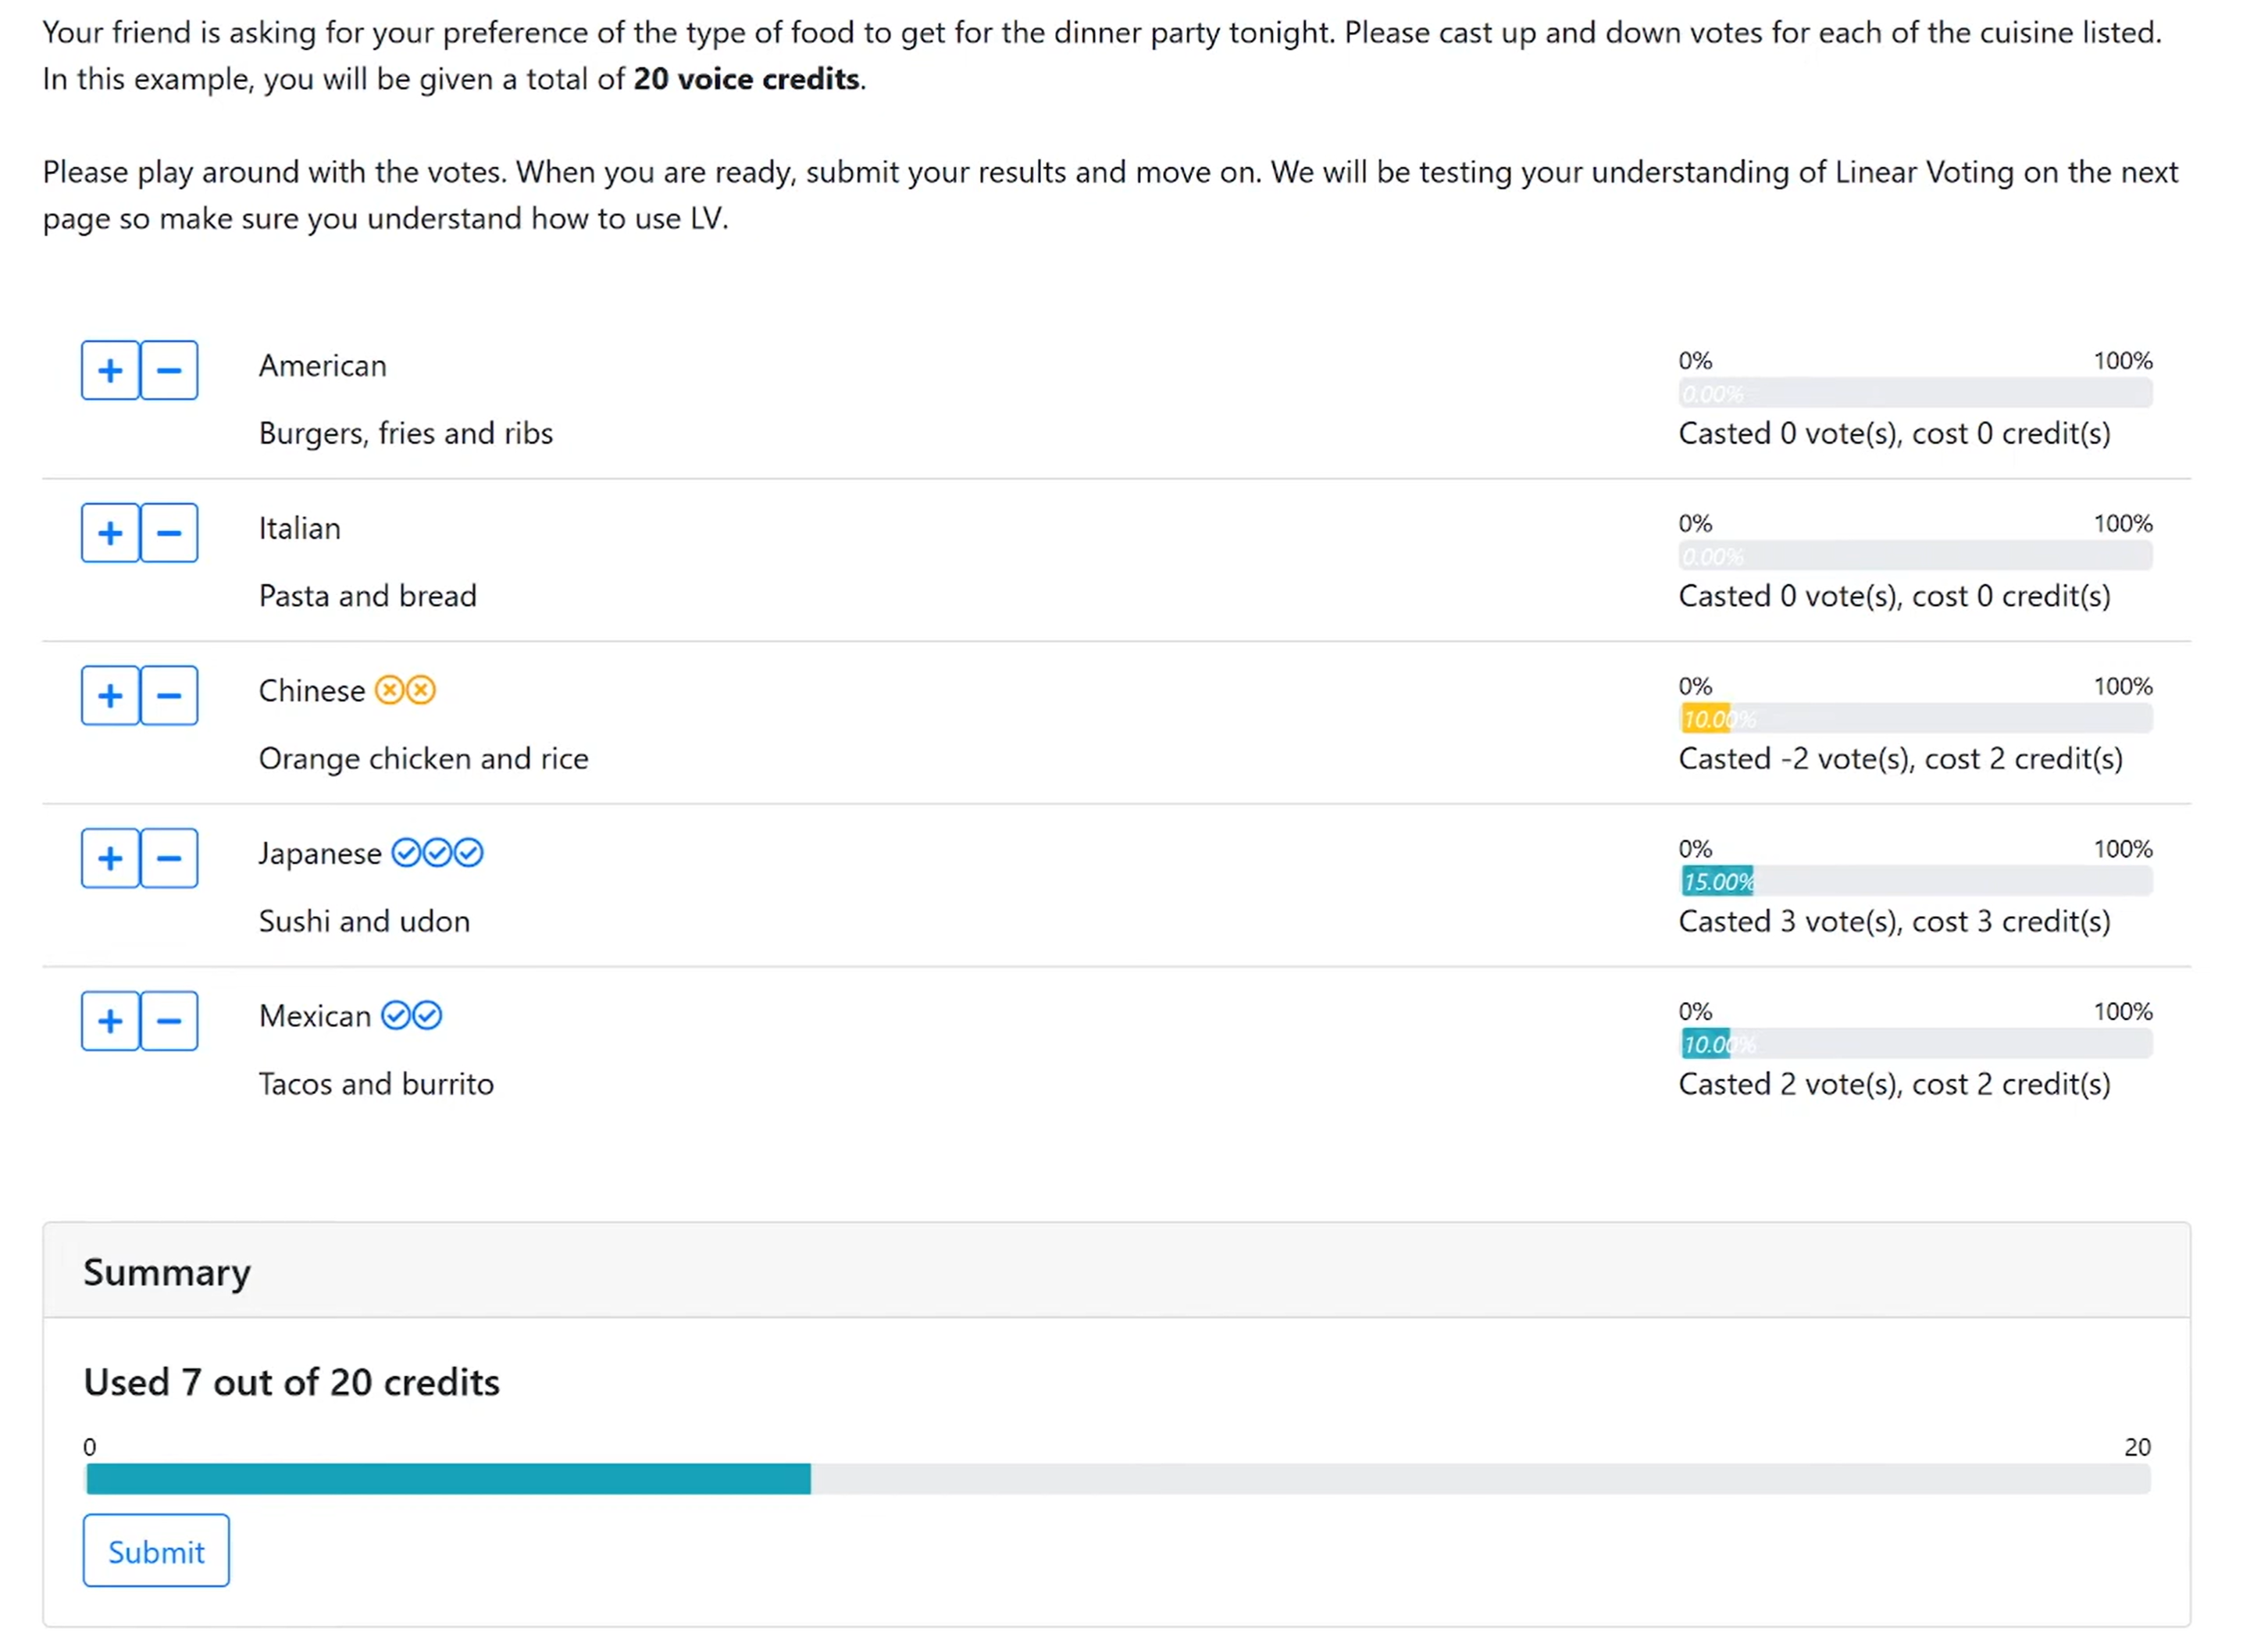
\includegraphics[width=\textwidth]{content/image/linear.png}
        \caption{Linear Survey (QS) Interface, each additional vote is $1$ credit}
        \label{fig:qs_interface}
    \end{subfigure}
    \hfill
    \begin{subfigure}{0.47\textwidth}
        \centering
        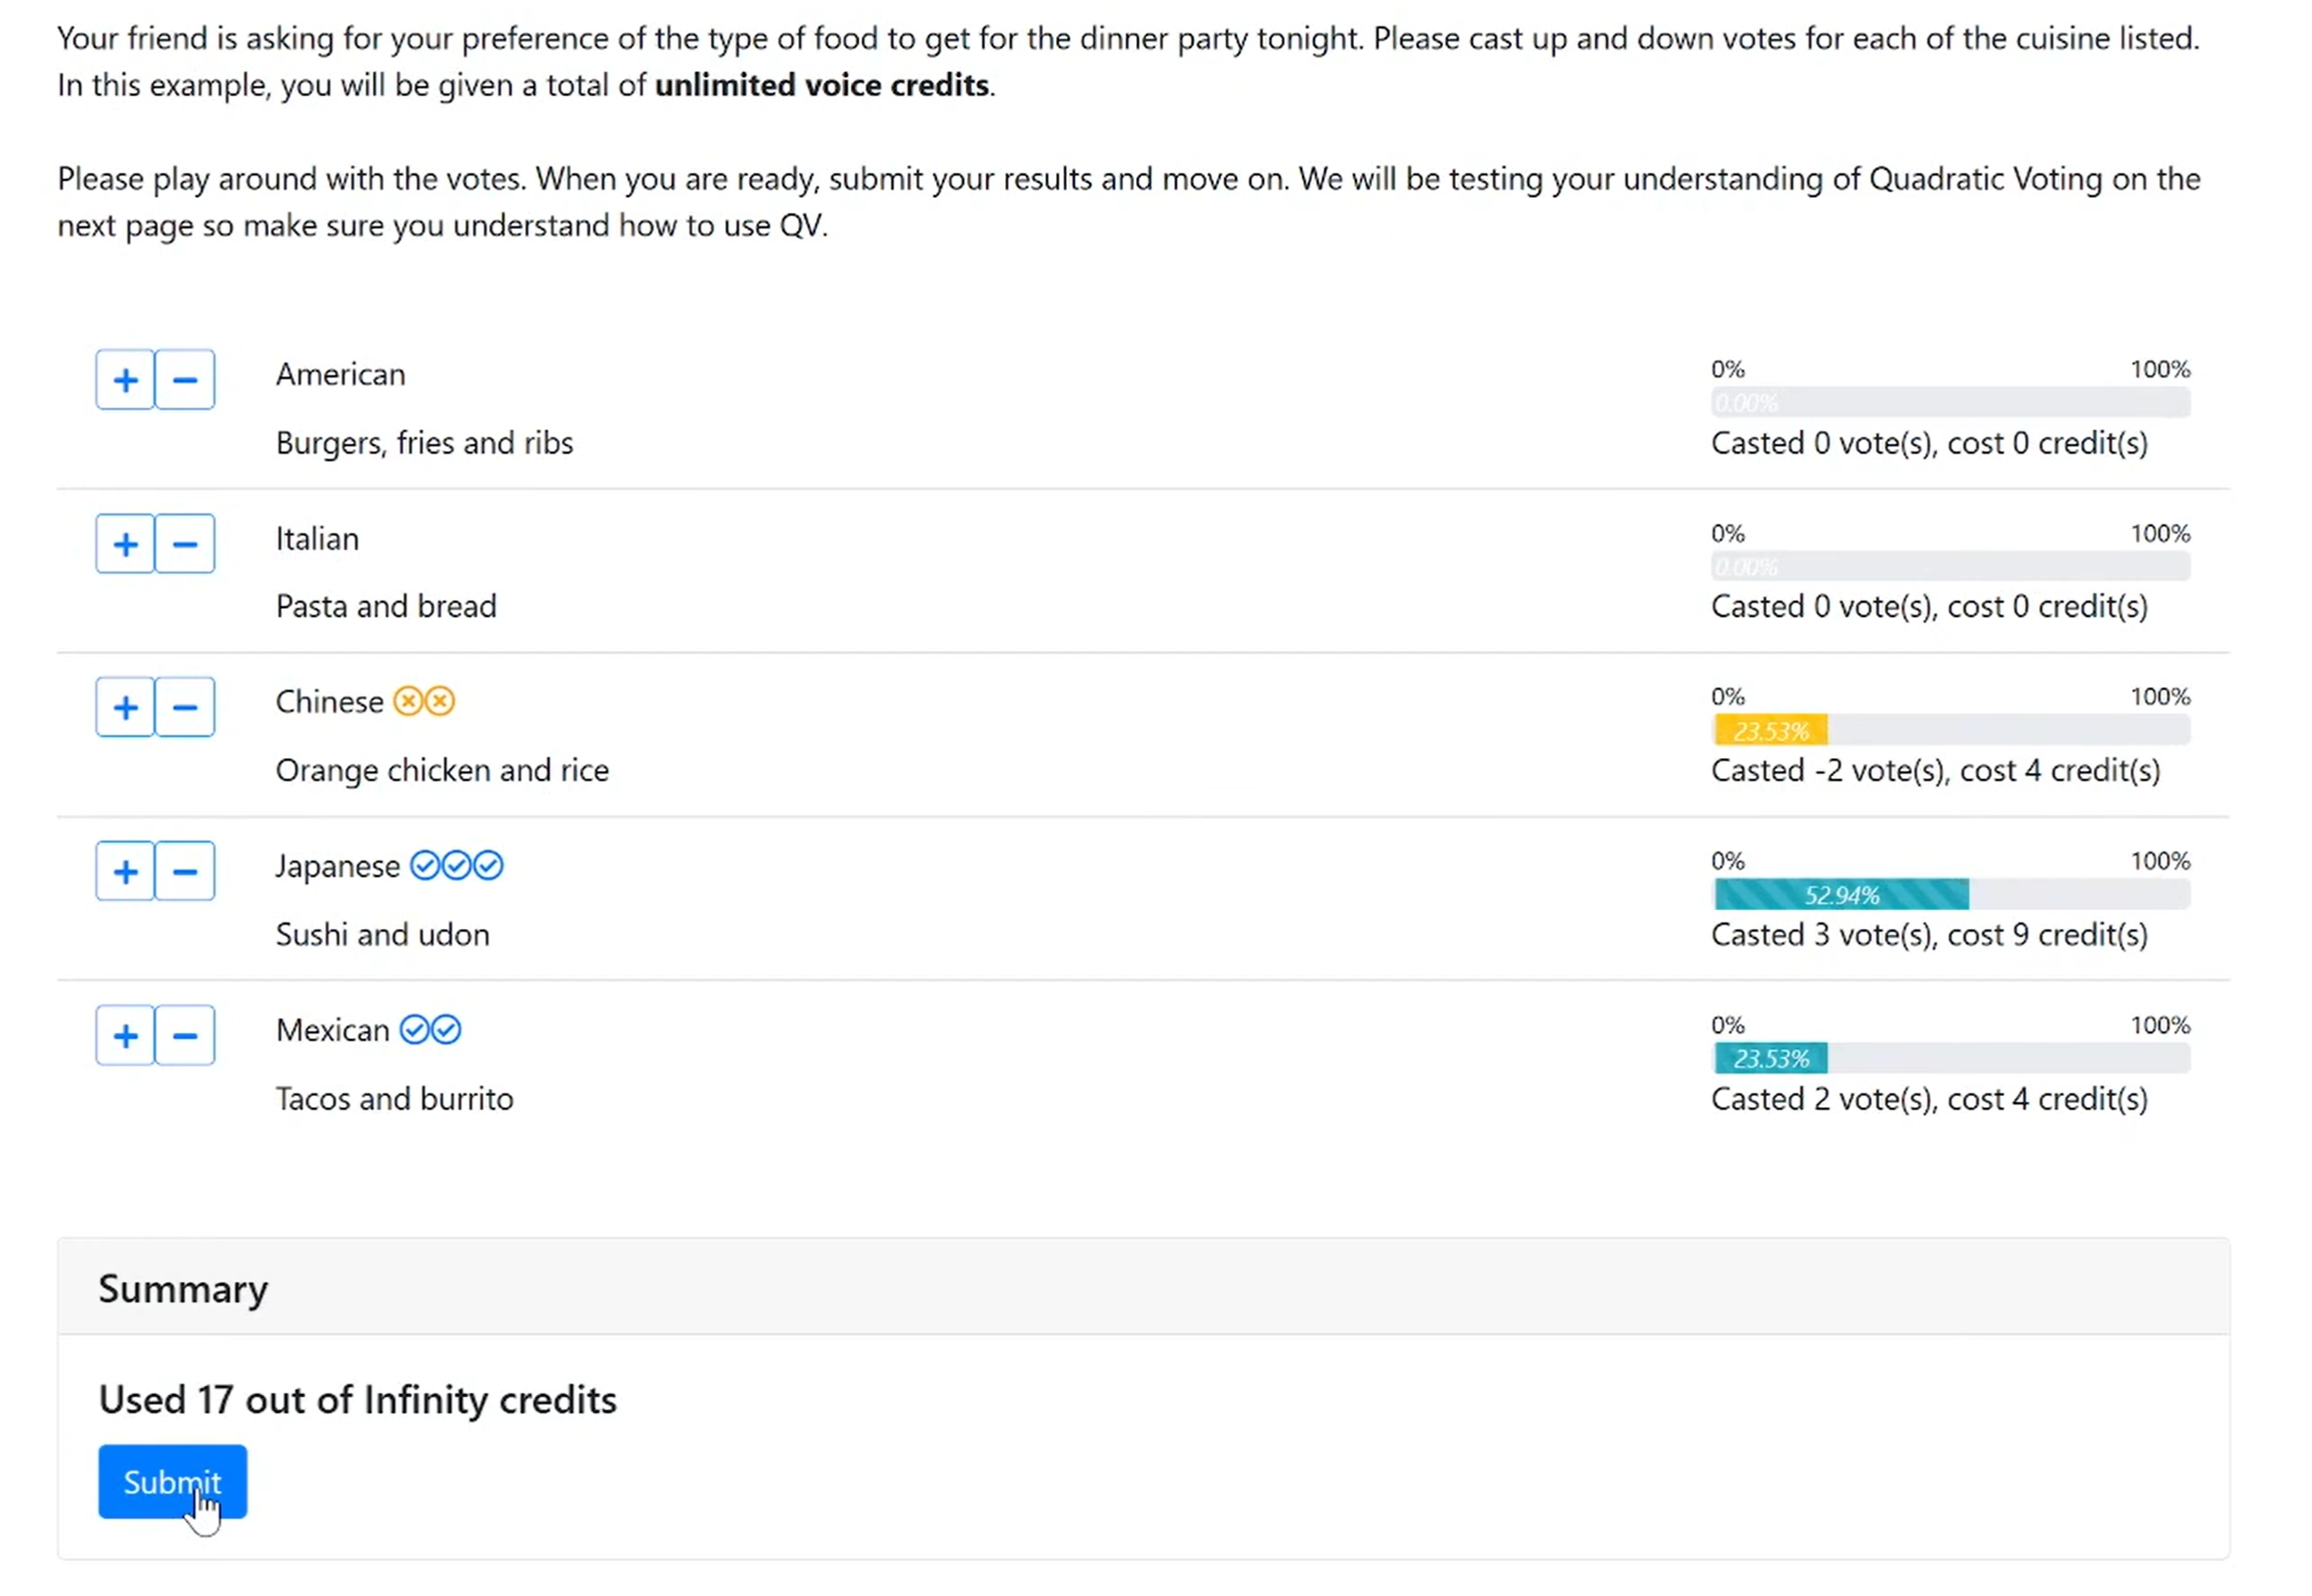
\includegraphics[width=\textwidth]{content/image/uqs.png}
        \caption{Unlimited Quadratic Survey (UQS) Interface, each additional vote is $n^2$ credits but does not have a budget constraint}
        \label{fig:css_interface}
    \end{subfigure}
    \caption{Survey interfaces for the two additional conditions. Both images are screenshots of the playground for participants to experience the surveying method before completing the actual survey tasks on societal issues.}
    \label{fig:extended_interface}
\end{figure}


\subsubsection{Filler task and donation}
After the survey, participants completed a filler task to prevent direct association with the issues and the charities listed on the donation task page. Participants 

\subsubsection{Debrief, and Compensation}
After the study, participants have a chance to read about the study's real purpose on the debrief page. Participants were compensated with \$1.50 for their time, and they were informed that they would receive an additional \$0.50 if they completed the study.

\subsubsection{Integrating prior data}
\citet{chengCanShowWhat2021} was the first study to evaluate the effectiveness of QS in relation to human behavior, offering an open dataset and open-source software that we replicated and extended. Their dataset contains 219 MTurk participants: 56 completed a Likert scale survey, 107 completed the QS36 survey, 108 completed QS108, and 111 completed QS324.

To facilitate our analysis, we differentiate between the number of votes allocated to each option (used in the original QS analysis) and the total credits spent on each option, which reflects the actual cost incurred under the quadratic cost function. To make this distinction clear, we refer to the credit-spent measures as QSC36, QSC108, and QSC324, corresponding to the cost-based modeling of QS36, QS108, and QS324 conditions.

Altogether, this study compares the elicited preferences from QS (vote-based), QSC (cost-based), LS (linear cost), UQS (QS without budget constraints), and Likert scale surveys, using participants' actual donation behavior as a behavioral baseline. These conditions are summarized in~\Cref{tbl:experiment_cond}.


\begin{table}[h]
    \centering
    \begin{tabular}{@{}lllp{9cm}@{}}
        \toprule
        \textbf{Condition} & \textbf{Budget} & \textbf{Cost Function} & \textbf{Description} \\
        \midrule
        Likert & – & – & A 5-point traditional ordinal-scale survey. \\ 
        \midrule
        Donation & – & – & Incentive-compatible donation task used as behavioral benchmark for validating expressed preferences. \\
        \midrule
        QS36   & 36   & Quadratic & \multirow{3}{9cm}{QS conditions with three different budgets ($O(K)$, $O(K^{1.5})$, $O(K^2)$). Participants expressed preferences by allocating votes, where the cost of each vote increased quadratically, deducted from the budget.} \\
        QS108  & 108  & Quadratic & \\
        QS324  & 324  & Quadratic & \\
        \midrule
        QSC36  & 36   & Quadratic & \multirow{3}{9cm}{Credits that participants contributed per option. Using the results from QS, QSC reflects the actual cost incurred per option to reflect perceived intensity of preference and explore alignment with donation outcomes.} \\
        QSC108 & 108  & Quadratic & \\
        QSC324 & 324  & Quadratic & \\
        \midrule
        LS18   & 18   & Linear    & \multirow{3}{9cm}{Linear-cost versions of QS with budgets scaled as $O(K)$, $O(K^{1.5})$, and $O(K^2)$. Participants expressed preferences by allocating votes, where the cost of each vote increased linearly, deducted from the budget.} \\
        LS54   & 54   & Linear    & \\
        LS162  & 162  & Linear    & \\
        \midrule
        UQS    & Unlimited & Quadratic & QS without a budget where participants expressed preferences by allocating votes, where the cost of each vote increased quadratically but there is not budget that they ahere to. \\
        \bottomrule
    \end{tabular}
    \caption{Summary of experimental and behavioral conditions, their cost structures, budget levels, and modeling purposes.}
    \label{tbl:experiment_cond}
\end{table}

\subsection{Quantitative Measures: Ordinal and Interval Measures}
\label{sec:quantitative_measures}
Two prior empirical studies compared elicited survey responses with behavioral outcomes, such as donation~\cite{chengCanShowWhat2021,cavaille2024cares} or letter length~\cite{cavaille2024cares}, as proxies for individual preferences. ~\citet{chengCanShowWhat2021} employed a Bayesian model to compute cosine similarity, measuring the alignment between participants' stated preferences and observed behaviors. ~\citet{cavaille2024cares} used linear regression to estimate the differences between the two.

While cosine similarity is useful for high-dimensional data, it presents interpretative challenges. For example, high alignment might result from large angular differences between vectors with identical rankings, while low alignment could stem from small angular differences between completely misaligned rankings. Linear regression, on the other hand, primarily captures correlations rather than causal relationships, limiting its explanatory power. Additionally, since each behavioral measure (e.g., donation, letter writing) represents a distinct task, it is difficult to compare relative preferences across options within the same participant.

Thus, in this study, we draw from prior literature when comparing multi-option survey instruments in breaking down and evaluating QS's ability to elicit the ordinal and interval scales seperately~\cite{collewetPreferenceEstimationPoint2023}. We construct Bayesian models for both analysis considering its transparent nature for interpretatinf posterior distributions beyond binary thresholds~\cite{mcelreath2018statistical, kay2016researcher}. We compared the 5 different conditions and describe the models in the following subsections.



\subsubsection{Pairwise Ordinal Measures}
\label{sec:ordinal_measures}
The first analysis, which we termed~\textbf{sign analysis}, focuses on understanding how the outcomes from different instruments align with participants' donation behavior in terms of preference order. To achieve this, we construct pairwise comparisons between the two sets. 

After removing participants that made zero donations, for each pairwise option on a survey, we modeled $y_i$ as the outcome variable of whether the order of the two options expressed through the instrument aligns with the order of the donated amount. In other words, our model learns how well does a given survey instrument capture the preference between two options with their donation amount? Since the possible outcome would be either align or misaligned ($\pm 1$), we modeled the outcome variable $y_i$ as a Bernoulli distribution (Equation~\ref{eq:ordinal_model_overall}).

\begin{equation}
    \label{eq:ordinal_model_overall}
    y_i \sim \text{Bernoulli}(\theta_i)
\end{equation}

\begin{equation}
    \label{eq:ordinal_model_logit}
    \text{logit}(\theta_i) = \alpha + \beta_c[C_i] + \beta_o[O_i] + \beta_p[P_i] + \beta_t[T_{1i}] + \beta_t[T_{2i}]
\end{equation}

The model $\theta_i$ is modeled as a logit function (Equation~\ref{eq:ordinal_model_logit}) between pairwise topics $T_{1i}$ and $T_{2i}$, which we control for the specific survey instrument $C_i$. We also control for the order for which participants complete the survey in the QS and LS conditions, denoted as $O_i$ and if so, if the participants was already aligned in a prior condition, $P_i$. The latter two experiment variable help control for potential learning effects since the two survey only differ in the number of provided budgets.

We applied a hiarchical approach to model these experimental variables with a non-centered parameterization~\cite{mcelreath2018statistical}. The hierarchical approach allows partial polling across different pairwise comparisons (e.g., considering how the participants consider the same pair of topics), while preventing overfitting. With so many experimental variables to model under this setup, we applied a non-centered parameterization allows the model to learn the distribution of the parameters from the data rather than being overly constrained by the priors~\cite{mcelreath2018statistical}. This yields more robust inferences, improves sampling efficiency and stability of the model.

This means that for each experimental variable, it follows Equation~\ref{eq:generic_non_center_hyper} where the different possible values of the variable are modeled as a normal distribution with mean $\mu_x$ and standard deviation $\sigma_x$.

\begin{equation}
    \label{eq:generic_non_center_hyper}
    x_i = \mu_x + \sigma_x \cdot \eta_i, \quad \eta_i \sim \mathcal{U}(0,1)
\end{equation}

Each sigma is drawn from a normal distribution with different hyperpriors for each variable. For example, $C_i$ which represents different experiment condition's survey instrument follow the following model:

\begin{align}
    \label{eq:generic_non_center_hyper_C}
    \beta_c[c_i] = \beta_a + \sigma_c \cdot \eta[c_i]\\
    \quad \sigma_c \sim \mathcal{U}(0,1)\\
    \quad \beta_a \sim \mathcal{N}(0, 0.5)\\
    \quad \eta[c_i] \sim \mathcal{N}(0, 1)
\end{align}

The rest of the experimental variables follows the same structure, with the only difference in the hyperprior distribution $\mu_x$. For example, the topics $T_{1i}$ and $T_{2i}$ has a hyperprior of $\mathcal{N}(0, 0.25)$, while the rest of the experimental variables have a hyperprior of $\mathcal{N}(0, 0.5)$. 

\subsubsection{Interval Measures}
\label{sec:interval_measures}
Following the ordinal comparisons,~\textbf{intensity model} assesses how effectively instruments capture the magnitude of preference differences between options. This model evaluates how well an instrument reflects varying degrees of preference along a continuum.

\paragraph{Aligning the variables} Constructing a intensity model to compare the different instruments is not trivial, since elicited values are continuous and others are ordinal. We took a conservative approach and model Likert scale and QS votes as ordinal values, especially when it is not clear whether participants considering the varying costs associated with different votes for the latter. In contrast, LS reflects incremental additions on a scale, and UQS does not have a limit; hence, both are treated as continuous. Rather than solely using final outcomes from each instrument, we also incorporated the cost of votes for QSs, assuming each dollar increment shares the same ``monetary'' value.

For instruments with bounded, continuous budgets (e.g., \textit{QSC\_36}, \textit{QSC\_108}, \textit{QSC\_324}) and linear surveys (\textit{LS\_18}, \textit{LS\_54}, \textit{LS\_162}), we project vote differences onto the $[0,1]$ interval. Since UQS lacks fixed bounds, we normalize the vote difference $V$ between two options $t_1$ and $t_2$ over the $k'$ options that the participant voted on:

\begin{equation}
    \text{Vote\_diff}_{UQS} 
    = (V_{t1} - V_{t2})/\textstyle\sum V_{k'}
\end{equation}
and apply the same normalization for UQS credits.

\paragraph{Projecting Ordinal values} 
To facilitate a direct comparison, we transform the ordinal results into an unobserved latent continuous variable using a Dirichlet-based ``cutpoint'' transformation. Specifically, for each instrument, we derive $K$ discrete ordinal \emph{difference} categories. For example, QS36 has 17 possible difference categories (ranging from $-8$ to $+8$)\footnote{Here, 36 credits can generate a largest difference of 5 votes vs.\ $-3$ votes.}. We then sample
\(\boldsymbol{\alpha}\) from a Dirichlet$(\mathbf{1}\cdot\delta)$ prior, where each of its $K-1$ positive components sums to 1:

\begin{equation}
    \boldsymbol{\alpha} \sim \mathrm{Dirichlet}\bigl(\mathbf{1}\cdot \delta\bigr)
\end{equation}

We modeled the distribution with $\delta=2$ as a weakly informative prior over the latent cutpoints. We pad this vector so that $\alpha_0 = 0$, then map each category $k$ to a latent continuous value:

\begin{equation}
    x_{\mathrm{latent}}^{(k)} = \sum_{j=0}^{k} \alpha_j.
\end{equation}

As $k$ increases, $x_{\mathrm{latent}}^{(k)}$ grows but remains within the $[0,1]$ interval, effectively assigning each ordinal category a continuous value. 

\paragraph{Projecting Donations} Finally, since donation amounts also vary by participant, we remove those who donated nothing and normalize each donation difference by the participant's total donation, mirroring our UQS approach. With these transformations, all experimental variables and outcomes lie in $[0,1]$, forming the basis for a \emph{hierarchical normal} model.

\paragraph{Modeling the outcome}
We seek to capture how an instrument \emph{predicts} the donation difference $y_i$ between two options. Conditional on a mean $\mu_i$, the outcome follows a normal distribution:

\begin{equation}
    \label{eq:intensity_normal}
    y_i \sim \mathcal{N}(\mu_i, \sigma_i).
\end{equation}

where $C_i$ denotes the survey instrument (Likert, QS, QS cost, LS, or UQS). We place a prior $\mathcal{N}(0,0.2)$ on the intercept $\beta_{c}[C_i]$ for each condition and use a non-centered parameterization~\cite{mcelreath2018statistical} to model condition-specific slopes:

\begin{equation}
    \beta_{\text{vote}}[C_i]
    \;=\;
    \beta_{\text{vote}\,\text{bar}}
    + \sigma_{\text{vote}}\,\eta_{\text{vote}}[C_i],
    \quad
    \beta_{\text{vote}\,\text{bar}}
    \sim
    \mathcal{N}(0,1),
    \quad
    \sigma_{\text{vote}}
    \sim
    \mathrm{Uniform}(0,1),
    \quad
    \eta_{\text{vote}}[C_i]
    \sim
    \mathcal{N}(0,1).
\end{equation}

These slopes, together with each instrument's intercept, determine how normalized vote differences $\text{VoteDiff}_i$ (either transformed ordinal or inherently continuous) map onto $y_i$. We also include an order effect $\beta_{o}[O_i]$ and topic intercepts $\beta_{t}[T_{1i}]$ and $\beta_{t}[T_{2i}]$, each following a non-centered prior with a Normal hyper-mean and a Uniform hyper-scale. Putting these elements together, the linear predictor is:

\begin{equation}
    \label{eq:intensity_linpred}
    \mu_i
    =
    \beta_{c}[C_i]
    +
    \beta_{\text{vote}}[C_i] \cdot \text{VoteDiff}_i
    +
    \beta_{o}[O_i]
    +
    \beta_{t}[T_{1i}]
    +
    \beta_{t}[T_{2i}].
\end{equation}

Each condition is then assigned its own standard deviation $\sigma_i=\beta_{\sigma}[C_i]$, where $\beta_{\sigma}[C_i]$ is drawn from an $\mathrm{Exponential}(1)$ prior. Hence, different instruments exhibit distinct variance in donation differences.

A hierarchical Bayesian approach ties all these parameters together via a non-centered parameterization:

\begin{equation}
    x_i
    =
    \mu_x
    + \sigma_x \cdot \eta_i,
    \qquad
    \eta_i
    \sim
    \mathcal{N}(0,1).
\end{equation}

Here, $\mu_x$ and $\sigma_x$ define the group-level mean and scale for each parameter type, and $x_i$ represents condition intercepts, slopes, order intercepts, or topic intercepts. By integrating condition, vote difference, order, and topic effects into a single hierarchical normal framework, our model provides a structured way to analyze how different survey instruments capture the intensity of preference differences.

